
\chapter{Návrh}\label{chap:design}

V~tejto kapitole predstavíme základný algoritmus a postupne sa budeme venovať jeho jednotlivým častiam. Budeme sa venovať metódam na zlepšenie úspešnosti klasifikátora a porovnáme rôzne prístupy. 
\bigskip

\section{Základný algoritmus}

Základný algoritmus (Obr. \ref{fig:base_alg}) vyzerá nasledovne: 
Najskôr sa získa obraz z webkamery. Ten sa potom spracuje a následne sa rozsegmentuje na jednotlivé pohybujúce sa objekty.
Každý z týchto segmentov sa predloží klasifikátoru, ktorý rozhodne, či daný segment je, alebo nie je ruka. Zo všetkých segmentou je vybratý ten, o ktorom si je klasifikátor najviac istý, že je ruka (a zároveň spĺňa danú hranicu). Z vybratého segmentu sa vypoičíta bod, ktorý je braný ako pozícia ruky. Tento bod je pridaný do postupnosti bodov, o ktorých sa ďalej rozhodne, či tvoria niektoré gesto. Ak klasifikátor gesta detekuje nejaké gesto, vykoná sa príslušná akcia - simulácia stlačenia niektorej klávesy - a postupnosť sa vymaže. Ak sa dlhšiu dobu v obraze nevykonala žiadna zmena a klasifikátor gesta nezistil žiadne gesto, postupnosť sa tiež vymaže.

\begin{figure}[htp]
    \centering
%    \includegraphics[scale=1]{img/00/extern-drive-encryption.1.mps}
    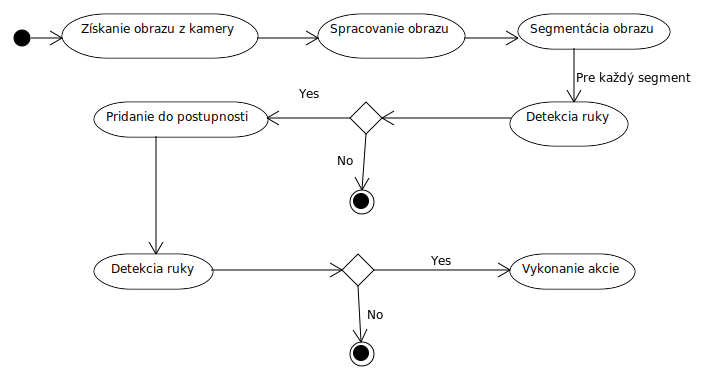
\includegraphics[width=\textwidth]{images/BaseAlgorithm}
%    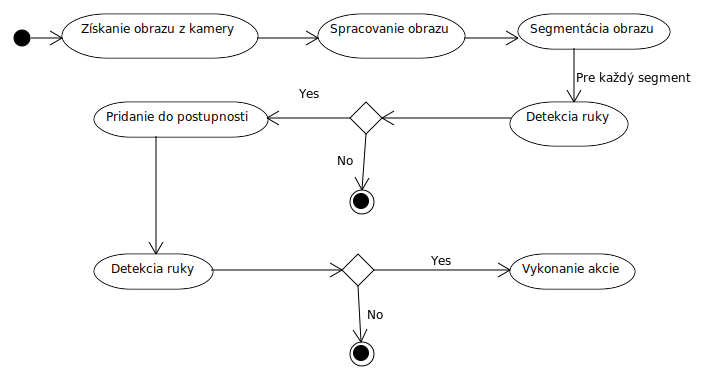
\includegraphics[scale=1]{images/BaseAlgorithm}
    \caption{Základný algoritmus}
    \label{fig:base_alg}
\end{figure}

\subsection{Predspracovanie a segmentácia}\label{chap:preprocess}

Základ pre predspracovanie a segmentáciu tvorí takzvaný \textbf{rozdielový obraz}. Rozdielový obraz je obraz, ktorý vznikne odčítaním 2 posebe idúcich čiernobielych obrázkov v absolútnej hodnote. Tento obraz obsahuje zmeny - pohybujúce sa objekty. Statické objekty sa tam teda nevyskytnú, čo nám umožní ich veľmi ľahko odfiltrovať. V tomto obraze sa vyskytnú obrysy pohybujúcich sa objektov, pretože ku zmenám dochádza najviac na hranách. Podľa rýchlosti pohybu môžu byť obrysy hrubšie, alebo tenšie. 
Našim cieľom je čo najlepšie zachytiť pohybujúcu sa ruku.

Dohodneme sa, že najmenšia zmena (žiadna) bude znázornená bielou a najväčšia čiernou. 

\subsubsection{Odfiltorvanie šumu}
Odfiltrovanie šumu zabezpečí hranica. Všetky pixle svetlejšie ako určitá konštanta, budú vykreslené bielou. Ideálna hranica je taká, ktorá potlačí šum, ale zachová čo najviac z ostatných zmien - čiže by mala byť najmenšia možná. Pohybujeme sa v odtieňoch šedej, čiže hodnoty $0\dots 255$. Praktické testy ukázali, že vhodnou hodnotou pre hranicu je 7.

\subsubsection{Rozpitie pixlov}

Kvôli segmentácii potrebujeme aby jednotlivé segmenty boli súvislé. Teda aby obrys ruky tvoril jeden celok.
Ľahko sa nám však môže stať, že obrys ruky je niekde prerušený - nedostatočná zmena, prípadne iné dôvody. Predpokladáme ale, že všetky časti jedného segmentu sú dostatočne blízko. Spojiť segmenty nám teda pomôže rozpitie pixlov. 

%TODO spravnu konštantu, spomenut rozlisenie
Z každého pixla spravíme štvorec s veľkosťou $11\times 11$.
Hodnota 11 pre stranu štvorca sa ukázala ako najvhodnejšia. 
Príliš veľké hodnoty spájajú aj časti, ktoré nepatria do toho istého segmentu, príliš malé zase nespoja časti, ktoré sú ďalej od seba.

\subsubsection{Segmentácia}\label{subsubsect:segment}
Rozpitý obrázok si teraz vieme predstaviť ako graf, pričom hrana je medzi každými 2 susediacimi pixlami (v štyroch smeroch). Segmentácia je vlastne len nájdenie komonentov v tomto grafe. Na to môžeme použiť napríklad prehľadávanie do šírky. Samozrejme musíme ešte nájsť opísaný obdĺžnik - stačí nájsť najľvejší, najpravejší, najvrchnejší a najspodnejší bod segmentu.

\subsection{Spracovanie segmentov}
Každý nájdený obdĺžnik sa naškáluje na veľkosť vstupu pre neurónovú sieť - v našom prípade $128\times 128$ - a normalizuje sa.

\section{Metódy na zlepšenie úspešnosti klasifikátora ruky}
\label{sect:metodyzlepseniaklasifikacie}

V tejto časti sa budeme zaoberať jednotlivými segmentami, ktoré budeme predkladať neurónovej sieti, aby nám povedala, či je to ruka, alebo nie.

\subsection{Pôvodný vs. rozdielový obrázok}
Nevýhodou rozdielového obrázka je, že zmena spôsobená pohybom sa v ňom vyskytne dvakrát. Raz na mieste, kam sa objekt posunul a raz na mieste odkiaľ sa posunul. Toto sme chceli eliminovať tak, že sa vyberie ruka z pôvodného obrázka podľa farby. Táto ruka tam bude vždy len raz. Bohužiaľ tento prístup mal viac zlých vlastností ako dobrých.

Pri vyberaní obrázka treba mať nastavené správne parametre, podľa ktorých sa rozhoduje čo pridať do výberu a čo nie. Tieto parametre veľmi závisia od osvetlenia. Navyše osvetlenie sa môže meniť pri pohybe ruky, čo veľmi stažuje nastavenie správnych parametrov. Pred použitím aplikácie by sa aplikácia musela nakalibrovať, čo znižuje komfort jej použitia.

Ďalší problém je správne tipnúť bod, ktorý patrí ruke, aby sa z neho mohla odštartovať selekcia. Pokiaľ by bola v danom obdĺžniku len dlaň, tak nie je až také ťažké sa správne trafiť - je takmer isté, že kúsok pod stredom obrázka bude dlaň. Bohužiaľ často sa stane, že užívaťeľ pohne nielen rukou, ale aj predlaktím a segmentačný algoritmus zaradí do segmentu aj predlaktie. Potom sa môže stať, že bod ruky netrafíme.

Rozhodujúcim problémom však bolo to, že úspešnosť siete na dátach, ktoré ani neobsahovali zle vybraté ruky bola aj tak nižšia ako u rozdielového obrázka. Preto sme sa rozhodli radšej pridať ďalšie dáta do trénovacej množiny pre rozdielové obrázky.

\subsection{Fourierova transformácia}
Fourierova transformácia zvykne často pomáhať, keď sa použie na predspracovanie dát pri trénovaní obrazových alebo zvukových vzoriek. Preto sme sa aj my rozhodli vyskúšať aký bude mať vplyv na úspešnosť.

Fourierova transformácia bola použitá na segment ako celok, potom bola prevedená do reálnych čísel pomocou absolútnej hodnoty a následne normalizovaná.

Konvergencia chyby pri trénovaní bola značne rýchlejšia a použitie transformácie umožnilo dosiahnuť menšiu chybu na trénovacej množine.

Úspešnosť na testovacej množine bola mierne nižšia.

\begin{table}[hp]
\catcode`\-=12 %kvoli babelu a pomlcke
\centering
\begin{tabular}{|l|c|c|c|c|}
\hline
 & \multicolumn{2}{c|}{\textbf{Malá sada}} & \multicolumn{2}{c|}{\textbf{Veľká sada}} \\ 
\cline{2-5}
 & \textbf{úspešnosť} & \textbf{chyba} & \textbf{úspešnosť} & \textbf{chyba}\\ \hline
\textbf{Rozdielový obr.} & & & &\\ \hline
\textbf{Pôvodný obr.} & & & &\\ \hline
\textbf{Rozdielový obr. FFT} & & & &\\ \hline
\textbf{Pôvodný obr. FFT} & & & &\\
\hline
\end{tabular}
\caption{Porovnanie úspešnosti NS pri rôznych dátach}
\end{table}
